\chapter{DSL for Logic Programming} % Main chapter title

\label{Chapter2} % Change X to a consecutive number; for referencing this chapter elsewhere, use \ref{ChapterX}

Questo secondo capitolo sarà dedicato alla presentazione del caso d'uso della libreria Scalaz realizzato in questo elaborato. Si è scelto di sfruttare alcune delle astrazioni offerte da Scalaz per implementare un DSL che imiti Prolog, in modo da fornire un supporto diretto alla programmazione logica.

Il DSL ha l'obiettivo di offrire un'interfaccia quanto più possibile semplice e simile a Prolog, ma che consenta di scrivere programmi direttamente in Scala. L'esecuzione di questi ultimi sarà basata sulla tecnica di risoluzione comunemente usata dai motori logici, ossia quella che prevede la costruzione di un SLD tree, e anch'essa sarà implementata con l'ausilio di Scalaz.

%----------------------------------------------------------------------------------------
%	SECTION 1
%----------------------------------------------------------------------------------------

\section{Available features}

Il DSL realizzato supporta una parte di quanto offerto dal linguaggio Prolog e, di seguito, sono riportate le funzionalità che mette a disposizione:

\begin{itemize}
\item Numeri di tipo \textit{Int} e \textit{Double} possono essere utilizzati per rappresentare rispettivamente i numeri interi e decimali presenti in Prolog.
\item Stringhe che iniziano con una lettera minuscola corrispondono a dei termini costanti, mentre le stringhe il cui primo carattere è costituito da una lettera maiuscola equivalgono a delle variabili.
\item Mentre in fase di compilazione tutte le stringhe vengono accettate in quanto termini, a run-time non sono considerate valide le stringhe vuote e quelle che non contengono solo lettere. Quest'ultimo vincolo è stato aggiunto per colmare il gap tra un linguaggio che è tipato staticamente (Scala) e uno che non lo è (Prolog). Sono infatti evitati i casi in cui si confronta un numero (ad esempio 1) e la stringa corrispondente (``1''), che in Prolog non possono verificarsi. Inoltre, escludere i caratteri speciali consente alle stringhe di non contenere delimitatori come ``,'' e ``)''.
\item È possibile creare un funtore usando il metodo \textit{apply} dell'oggetto \textit{Struct} e specificando il nome del funtore, che deve essere una stringa non vuota, contenere solo lettere e iniziare con una lettera minuscola.
\item A sua volta, un funtore offre un metodo \textit{apply} che accetta un numero variabile di termini e restituisce un termine composto. È previsto un errore se non viene passato nessun termine quando si usa un funtore. Se si divide la definizione del funtore dalla creazione del termine composto, questa operazione è molto simile a ciò che si farebbe in Prolog.

\lstinputlisting{code/PrologCompound.scala}
\item In modo speculare a quanto visto per funtori e termini composti, il DSL offre l'oggetto \textit{Predicate} con cui è possibile inizializzare dei predicati che a loro volta sono utilizzabili per la creazione di fatti.
\item Sono supportate le regole, che possono essere definite a partire da un fatto chiamando il metodo :- e passando ad esso un numero variabile di fatti (previsto un errore in assenza di argomenti). Il fatto su cui viene chiamato il metodo costituisce la testa della regola, mentre gli argomenti corrispondono al suo corpo. La notazione infissa disponibile in Scala rende naturale la definizione di regole, ma è importante ricordare che si tratta di una chiamata di metodo e quindi, se il corpo della regola contiene più fatti, è necessario racchiuderli tra parentesi.

\lstinputlisting{code/PrologRule.scala}
\item Gli elementi descritti finora consentono di definire un programma Prolog, che è costituito da una serie di clausole corrispondenti alla teoria (che possono essere fatti o regole) e da un insieme di fatti che rappresentano i goal. Per la loro risoluzione il DSL fornisce un oggetto \textit{Engine}, che costituisce il motore logico condiviso nell'applicazione.
\item \textit{Engine} consente di aggiungere e resettare la teoria del programma, tramite i metodi \textit{addTheory} e \textit{resetTheory}, e fornisce due modalità di risoluzione alternative (le stesse offerte da tuProlog), grazie ai metodi \textit{solve} e \textit{solveAll}, con cui è possibile risolvere uno o più goal. Nella prima modalità la computazione procede finché non viene trovata una soluzione e, in quel momento, l'utente può scegliere se interrompere l'esecuzione o proseguire fino alla soluzione successiva. Nella seconda modalità, invece, sono esplorate tutte le possibili alternative. È inoltre possibile abilitare la stampa dell'albero di esecuzione del programma.
\item Come si può facilmente intuire, ogni chiamata di \textit{solve} o \textit{solveAll} corrisponde all'esecuzione di un programma Prolog. Per ognuna di esse \textit{Engine} porta a termine un procedimento di validazione dell'input, che prevede la mancata esecuzione del programma in caso di errori nei suoi elementi (variabili, termini costanti, termini composti, fatti o regole) e la restituzione di un report contenente tutti gli errori trovati.
\end{itemize}

Per utilizzare il DSL è sufficiente specificare gli statement \textit{import prologz.dsl.\_}, con cui si ottengono tutti i costrutti visti in precedenza, \textit{import prologz.dsl.ClauseImplicits.\_} e \textit{import prologz.dsl.TermImplicits.\_}, che mettono a disposizione le conversioni implicite necessarie per la definizione di termini, fatti e regole.

\begin{figure}[th]
\centering
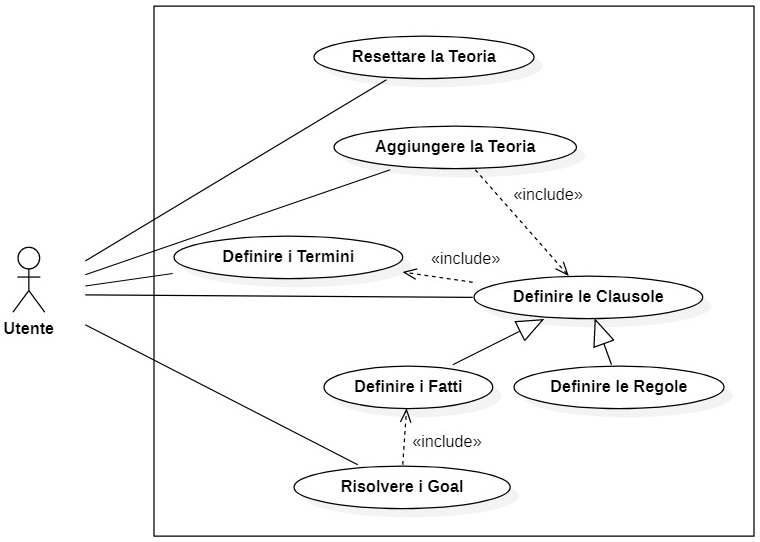
\includegraphics[scale=0.79]{images/DiagramUseCase}
\decoRule
\caption[DiagramUseCase]{Diagramma dei casi d'uso in cui è rappresentata l'interazione tra il DSL e i suoi utenti (sviluppatori che lo usano)}
\end{figure}

%----------------------------------------------------------------------------------------
%	SECTION 2
%----------------------------------------------------------------------------------------

\section{Implementation details}

Il codice realizzato è suddiviso in due package: \textit{prologz.dsl}, che contiene la definizione degli elementi di Prolog supportati dal DSL e gli strumenti offerti agli utilizzatori, e \textit{prologz.resolution}, destinato a ciò che è necessario per la risoluzione dei programmi. I principali componenti del DSL sono i seguenti:

\begin{itemize}
\item \textit{Engine}, che costituisce il motore logico messo a disposizione.
\item \textit{Validation}, un'entità ``posseduta'' da \textit{Engine} e grazie a cui è possibile eseguire il procedimento di validazione dei programmi Prolog.
\item \textit{PrologTree}, che consente di creare e navigare l'albero di risoluzione.
\item \textit{Substitution}, ossia la modellazione del concetto di sostituzione.
\item \textit{RichClause}, usato da \textit{PrologTree} e che offre ad una clausola (fatto o regola) la possibilità di essere unificata con un altro fatto.
\item \textit{RichElement}, le cui implementazioni forniscono la possibilità di applicare una sostituzione, rinominare o ottenere le variabili presenti in diversi elementi, come ad esempio fatti o regole.
\end{itemize}

\begin{figure}[th]
\centering
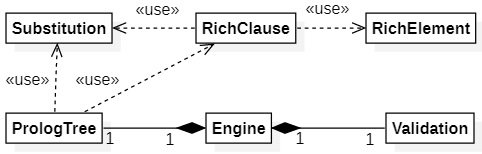
\includegraphics[scale=1.02]{images/DiagramDesign}
\decoRule
\caption[DiagramDesign]{Design ad alto livello del DSL}
\end{figure}

\subsection{Program validation}

Per quanto riguarda i costrutti di Prolog supportati dal DSL, si è scelto di modellare i termini come case class che definiscono dei sottotipi del trait \textit{Term}: \textit{Atom[A]} per i termini costanti e i numeri (interi o decimali), \textit{Variable} per le variabili e \textit{Struct} per i termini composti. Allo stesso modo, le case class \textit{Fact} e \textit{Rule} corrispondono ai fatti e alle regole ed estendono il trait \textit{Clause}. Funtori e predicati sono invece rappresentati tramite stringhe taggate, rispettivamente \textit{String @@ Functor} e \textit{String @@ Predicate}, poiché si tratta semplicemente di elementi che devono essere in grado di incapsulare una stringa.

\begin{figure}[th]
\centering
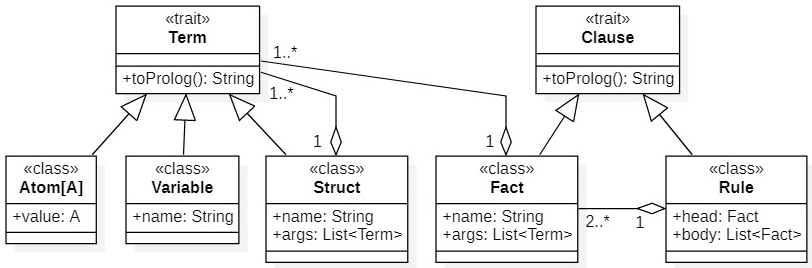
\includegraphics[scale=0.86]{images/DiagramClauseTerm}
\decoRule
\caption[DiagramClauseTerm]{Diagramma delle classi per termini e clausole}
\end{figure}

Le modalità standard per la costruzione di valori di questi tipi sono però nascoste agli utilizzatori del DSL, che hanno a disposizione solo quanto visto nella sezione precedente per definire gli elementi del programma Prolog. Il motivo di questa scelta è evidente se si considerano le definizioni dei metodi \textit{addTheory}, \textit{solve} e \textit{solveAll} presenti in \textit{Engine}: essi accettano rispettivamente \textit{PzValidation[Clause]*} e \textit{PzValidation[Fact]*} (invece di \textit{Clause*} e \textit{Fact*}).

\textit{PzValidation[A]} è un semplice type alias che corrisponde a \textit{ValidationNel[String @@ InputError, A]}, dove String @@ InputError è un tipo usato per rappresentare gli errori nella definizione del programma Prolog. Tutti gli elementi presenti al suo interno, a partire dai più semplici come termini costanti e variabili, sono creati come istanze di \textit{PzValidation[A]} (A è il tipo che rappresenta quell'elemento) e possono quindi incapsulare errori nella loro definizione.

In questo modo, sfruttando la possibilità di accumulare gli errori offerta dal costrutto \textit{Validation} e la sintassi proposta dall'\textit{Applicative Builder} per gestire i casi di successo, è stato realizzato il meccanismo di validazione dell'input descritto in precedenza. In caso di errori viene semplicemente restituito un report, evitando di lanciare eccezioni e di interrompere l'esecuzione.

Un altro vantaggio si ha nel caso di più programmi Prolog da eseguire: se sono presenti errori in alcuni di essi, gli altri vengono risolti normalmente.

\lstinputlisting[caption=Metodi per la creazione di \textit{PzValidation[Term]} e per la concatenazione di \textit{PzValidation[Clause]} e di \textit{PzValidation[Fact]}]{code/PrologValidation.scala}

\subsection{Prolog execution}

L'esecuzione dei programmi Prolog è basata sulla costruzione dell'SLD tree, un albero in cui ogni nodo corrisponde ad una coppia contenente sia i goal che devono ancora essere risolti sia una sostituzione che rappresenta una soluzione valida per i goal che sono stati risolti fino a quel momento.

Nella programmazione logica, una sostituzione è definita come una mappa finita da variabili a termini e, quindi, si è scelto di rappresentarla tramite l'alias \textit{type Substitution = Map[Variable, Term]}. Il meccanismo di risoluzione di Prolog prevede che più sostituzioni debbano poter essere unite in un'unica sostituzione avente come effetto l'esecuzione sequenziale delle varie sostituzioni considerate: dati due goal R1 e R2 risolti rispettivamente dalle sostituzioni A e B, la loro soluzione sarà rappresentata da una sostituzione AB con effetto equivalente all'applicazione di A seguita dall'applicazione di B.

La politica di combinazione delle mappe offerta da Scalaz con l'implementazione di \textit{Monoid[Map]} non è adatta alle sostituzioni, perché le unisce semplicemente e sovrascrive i valori che compaiono più volte. Ad esempio, date due sostituzioni A=\{X/2,Y/X\} e B=\{X/3\}, si ottiene come risultato AB=\{Y/X,X/3\} mentre la sostituzione equivalente è AB=\{X/2,Y/3\}.

Perciò è stata definita una nuova implementazione di \textit{Monoid[Substitution]}, in cui aggiungere una sostituzione ad un'altra equivale ad applicarla a tutti i termini nelle relazioni variabile/termine della prima sostituzione. In questo modo è sufficiente usare l'operatore |+| per unire le sostituzioni ma, affinché il procedimento funzioni, è necessario che la sostituzione inziale sia un'identità in cui ogni variabile presente nei goal è associata a sé stessa.

\newpage

\lstinputlisting[caption={Definizione di \textit{SubstitutionMonoid}, il metodo \textit{substitute} consente (utilizzando un implicito) di applicare una sostituzione ad una lista di termini}]{code/PrologSubstitution.scala}

Dopo aver stabilito come rappresentare e unire le sostituzioni, è stato possibile implementare il meccanismo di risoluzione. Esso prevede che tutti i programmi Prolog siano convertiti in alberi SLD, realizzati e gestiti sfruttando le strutture dati \textit{Tree} e \textit{TreeLoc} offerte da Scalaz. Per ogni nodo dell'albero, oltre ai goal da risolvere e alla sostituzione eseguita, è memorizzata una lista di clausole che rappresentano la parte di teoria non ancora considerata.

Inizialmente l'albero di risoluzione è costituito da un solo nodo contenente la teoria del programma, i goal e una sostituzione identità. In seguito questo nodo, quello attualmente selezionato nel \textit{TreeLoc} dell'albero, viene passato ad una procedura ricorsiva (implementata dal metodo \textit{navigatePrologTree} e richiamata grazie a \textit{searchPrologTree}) che si comporta come segue:

\begin{itemize}
\item Se la teoria e i goal non sono vuoti, la prima clausola presente nella teoria viene rimossa dal nodo attuale perché, al termine della chiamata in corso, non dovrà più essere considerata. Si esegue quindi l'unificazione (disponibile grazie al metodo \textit{unify}) tra questa clausola e il primo goal.

Se ha successo, l'unificazione restituisce la sostituzione corrispondente alla soluzione e i goal rimanenti: nel caso di un fatto si tratta degli altri goal dopo l'applicazione della sostituzione, mentre nel caso di una regola è considerato anche il suo corpo. Viene quindi aggiunto un nodo all'albero (ultimo figlio del nodo corrente) contenente tutte le clausole di teoria previste dal programma (possono essere utilizzate di nuovo tutte per risolvere gli altri goal), i goal rimanenti e l'unione tra la sostituzione presente nel nodo corrente e quella ottenuta con l'unificazione. La procedura è chiamata ricorsivamente su questo nodo.

Al contrario, se l'unificazione non ha successo, la procedura viene chiamata ricorsivamente sul nodo corrente. In questo modo, è possibile tentare di unificare il primo goal con tutte le clausole della teoria.
\item Se la teoria è vuota ma devono ancora essere risolti uno o più goal ed è definito il padre del nodo corrente, è facile capire che quest'ultimo rappresenta una foglia in cui non è stata trovata nessuna soluzione. Perciò, viene eseguito automaticamente il \textit{backtracking} e la procedura è richiamata ricorsivamente sul nodo padre del nodo corrente.
\item Se non si verificano i due casi precedenti, il nodo corrente può rappresentare una foglia contenente una soluzione valida o la radice (e quindi la fine della computazione). La procedura termina restituendo in entrambi i casi il nodo corrente e offre così la possibilità di interrompere la computazione ogni volta che viene trovata una soluzione.
\item Il metodo \textit{searchPrologTree} permette di riprendere l'esplorazione dell'albero di risoluzione da qualsiasi punto, eseguendo il \textit{backtracking} se il nodo corrente non è la radice. La sua esecuzione ripetuta consente di trovare tutte le soluzioni disponibili per un programma Prolog.
\end{itemize}

\lstinputlisting[caption=Costruzione dell'albero di risoluzione Prolog]{code/PrologTree.scala}

\subsection{Unification}

Finora l'unificazione è stata vista come un procedimento ``black box'', che confronta un fatto o una regola (ossia una clausola appartenente alla teoria) con un altro fatto (goal) e, in caso di successo, restituisce una sostituzione corrispondente al risultato e i goal che devono ancora essere risolti.

L'implementazione dell'unificazione è contenuta nel metodo \textit{unify}, disponibile grazie agli impliciti (in modo simile a quanto fatto da Scalaz con la \textit{method injection}) su qualunque clausola. In base al tipo di clausola (fatto o regola), il procedimento è differente. In entrambi i casi è molto importante il ruolo dei goal restanti da eseguire, che sono modificati in base al risultato dell'unificazione. Perciò si è scelto di implementare l'unificazione basandosi sul trasformatore della state monad, \textit{StateT}, in cui lo stato è costituito dai goal che non sono ancora stati risolti ed è prevista l'opzionalità.

L'unificazione di due fatti prevede le seguenti operazioni:

\begin{enumerate}
\item Controllare se il fatto e il goal sono caratterizzati dallo stesso nome e dalla stessa arità e, in caso contrario, restituire un esito negativo.
\item Rinominare le variabili presenti nel fatto appartenente alla teoria, in modo che non vi siano né variabili comuni al goal con cui deve essere unificato né variabili comuni agli altri goal da risolvere. Questo perché se una variabile compare due volte nei goal (anche in goal differenti), deve essere associata ad uno stesso termine. Si tratta però di un vincolo che deve poter essere espresso solo in fase di definizione dei goal, e che non può derivare dall'unificazione con una clausola della teoria.
\item Unificare gli argomenti del fatto e del goal, seguendo le regole previste da Prolog per l'unificazione di termini. In caso di successo, mantenere la sostituzione ed eliminare il goal corrente da quelli da risolvere.
\item Applicare la sostituzione trovata ai goal che devono ancora essere risolti e restituire una tupla contenente sia questi sia la sostituzione. È importante notare che, grazie al comportamento \textit{first-fail} di \textit{StateT}, questa operazione non viene eseguita se l'unificazione ha esito negativo.
\end{enumerate}

Unificare una regola con un fatto è invece un procedimento leggermente più complesso, che è caratterizzato dalle seguenti operazioni:

\begin{itemize}
\item Replicare i primi tre passi previsti per l'unificazione di fatti. In particolare: eseguire il controllo sulla testa della regola e sul goal, rinominare sia la testa sia il corpo della regola evitando le variabili contenute nei vari goal e unificare gli argomenti della testa della regola e del goal.
\item Se l'unificazione ha successo, aggiungere ai goal da risolvere i fatti presenti nel corpo della regola. Prima è però necessario rinominare le variabili presenti nel corpo della regola ma non nella sua testa (le variabili in testa sono già state considerate), facendo in modo che non compaiano anche negli altri goal. Si evita così l'aggiunta di vincoli inesistenti che possono precludere la corretta risoluzione del programma.
\item Infine, come nel punto 4 visto per l'unificazione di fatti, si applica la sostituzione trovata ai goal che devono ancora essere risolti e viene restituita una tupla contenente sia questi sia la sostituzione.
\end{itemize}

%----------------------------------------------------------------------------------------
%	SECTION 3
%----------------------------------------------------------------------------------------

\section{Final remarks}

Il numero di funzionalità presenti in Prolog e supportate dal DSL è ancora limitato, ma ritengo che possa costituire una base valida per estensioni che supportino altre funzionalità. Ad esempio, non dovrebbe essere eccessivamente complicato aggiungere il supporto alle liste e l'operatore ``'!''.

Attualmente l'interazione prevista consente soltanto di visualizzare a riga di comando i risultati dei programmi risolti. Sarebbe però semplice modificare l'interfaccia presente in \textit{Engine} e ottenere le soluzioni sotto forma di valori tipati, in modo da facilitare l'integrazione con altre applicazioni (ad esempio, con giochi che definiscono la propria logica utilizzando Prolog).

A mio parere, Scalaz si è rivelato un ottimo strumento ed ha rappresentato un valido ausilio per la realizzazione di questo progetto. Le strutture funzionali che offre hanno infatti consentito di implementare meccanismi complessi in modo ancor più naturale e semplice di quanto possibile in Scala.

Come visto in precedenza, nell'implementazione del DSL sono state fondamentali anche le caratteristiche messe a disposizione nativamente da Scala, quali ad esempio case class, pattern matching e conversioni implicite. In particolare, grazie a queste ultime è stato possibile consentire di scrivere in Scala programmi molto simili a quelli Prolog ed è stata evidente l'importanza ricoperta da questi strumenti nella realizzazione di un qualsiasi DSL.

Infine, i test realizzati con ScalaTest (e presenti nel package \textit{test.scala.prologz}) hanno consentito di verificare il funzionamento di quanto implementato e costituiscono una valida specifica del comportamento del sistema.
